\documentclass[submit]{../harvardml}

\course{CS1810-S25}
\assignment{Assignment \#1}
\duedate{11:59pm ET, February 14, 2025} 

\usepackage[OT1]{fontenc}
\usepackage[colorlinks,citecolor=blue,urlcolor=blue]{hyperref}
\usepackage{graphicx}
\usepackage{caption}
\usepackage{enumitem}
\usepackage{soul}
\usepackage{amsmath}
\usepackage{amssymb}
\usepackage{color}
\usepackage{todonotes}
\usepackage{listings}
\usepackage{../common}
\usepackage{framed}
\usepackage{float}
\usepackage{ifthen}
\usepackage{bm}
\usepackage{mathtools}
\usepackage{colortbl} 

\usepackage[mmddyyyy,hhmmss]{datetime}

\definecolor{verbgray}{gray}{0.9}

\lstnewenvironment{csv}{
  \lstset{backgroundcolor=\color{verbgray},
  frame=single,
  framerule=0pt,
  basicstyle=\ttfamily,
  columns=fullflexible}}{}

 \DeclareMathOperator*{\limover}{\overline{lim}}

%%%%%%%%%%%%%%%%%%%%%%%%%%%%%%%%%%
%% Solution environment
\usepackage{xcolor}
\usepackage{comment}
\newenvironment{solution}
  {\color{blue}\section*{Solution}}
{}
%%%%%%%%%%%%%%%%%%%%%%%%%%%%%%%%%%



\begin{document}
\begin{center}
  {\Large Homework 1: Regression}\\
\end{center}

\subsection*{Introduction}
This homework is on different three different forms of regression:
kernelized regression, nearest neighbors regression, and linear
regression.  We will discuss implementation and examine their
tradeoffs by implementing them on the same dataset, which consists of
temperature over the past 800,000 years taken from ice core samples.

The folder \verb|data| contains the data you will use for this
problem. There are two files:
\begin{itemize}
  \item \verb|earth_temperature_sampled_train.csv|
  \item \verb|earth_temperature_sampled_test.csv|
\end{itemize}

Each has two columns.  The first column is the age of the ice core
sample.  The second column is the approximate difference in a year's temperature (K)
from the average temperature of the 1,000 years preceding it. The temperatures were retrieved from ice cores in
Antarctica (Jouzel et al. 2007)\footnote{Retrieved from
  \url{https://www.ncei.noaa.gov/pub/data/paleo/icecore/antarctica/epica_domec/edc3deuttemp2007.txt}

  Jouzel, J., Masson-Delmotte, V., Cattani, O., Dreyfus, G., Falourd,
  S., Hoffmann, G., … Wolff, E. W. (2007). Orbital and Millennial
  Antarctic Climate Variability over the Past 800,000 Years.
  \emph{Science, 317}(5839), 793–796. doi:10.1126/science.1141038}.

The following is a snippet of the data file:

\begin{csv}
  # Age, Temperature
  399946,0.51
  409980,1.57
\end{csv}

\noindent And this is a visualization of the full dataset:
\begin{center}
  \includegraphics[width=.8\textwidth]{img_input/sample_graph}
\end{center}
\noindent


\textbf{Due to the large magnitude of the years, we will work in terms
  of thousands of years BCE in these problems.} This is taken care of
for you in the provided notebook.






\subsection*{Resources and Submission Instructions}
If you find that you are having trouble with the first couple
problems, we recommend going over the fundamentals of linear algebra
and matrix calculus (see links on website).  The relevant parts of the
\href{https://github.com/harvard-ml-courses/cs181-textbook/blob/master/Textbook.pdf}{cs181-textbook
  notes are Sections 2.1 - 2.7}.  We strongly recommend reading the
textbook before beginning the homework.

We also encourage you to first read the
\href{http://users.isr.ist.utl.pt/~wurmd/Livros/school/Bishop\%20-\%20Pattern\%20Recognition\%20And\%20Machine\%20Learning\%20-\%20Springer\%20\%202006.pdf}{Bishop
  textbook}, particularly: Section 2.3 (Properties of Gaussian
Distributions), Section 3.1 (Linear Basis Regression), and Section 3.3
(Bayesian Linear Regression). (Note that our notation is slightly
different but the underlying mathematics remains the same!).

\textbf{Please type your solutions after the corresponding problems
  using this \LaTeX\ template, and start each problem on a new page.}
You may find the following introductory resources on \LaTeX\ useful:
\href{http://www.mjdenny.com/workshops/LaTeX_Intro.pdf}{\LaTeX\ Basics}
and
\href{https://www.overleaf.com/learn/latex/Free_online_introduction_to_LaTeX_(part_1)}{\LaTeX\ tutorial
  with exercises in Overleaf}

Homeworks will be submitted through Gradescope. You will be added to
the course Gradescope once you join the course Canvas page. If you
haven't received an invitation, contact the course staff through Ed.

\textbf{Please submit the writeup PDF to the Gradescope assignment
  `HW1'.} Remember to assign pages for each question.

\textbf{Please submit your \LaTeX file and code files to the
  Gradescope assignment `HW1 - Supplemental'.} Your files should be
named in the same way as we provide them in the repository,
e.g. \texttt{hw1.pdf}, etc.

%%%%%%%%%%%%%%%%%%%%%%%%%%%%%%%%%%%%%%%%%%%%%
% Problem 1
%%%%%%%%%%%%%%%%%%%%%%%%%%%%%%%%%%%%%%%%%%%%%
\begin{problem}[kNN and Kernels, 35pts]

You will now implement two non-parametric regressions to model temperatures over time.  
% For this problem, you will use the \textbf{same dataset as in Problem 1}.

\vspace{0.5cm}
\noindent\emph{Make sure to include all required plots in your PDF. Passing all test cases does not guarantee that your solution is correct, and we encourage you to write your own. }

\begin{enumerate}
\item 
 Recall that kNN uses a predictor of the form
\[
  f(x^*) = \frac{1}{k} \sum_n y_n \mathbb{I}(x_n \texttt{ is one of k-closest to } x^*),
\]
where $\mathbb{I}$ is an indicator variable. 
\begin{enumerate}

  \item The kNN implementation \textbf{has been provided for you} in the notebook. Run the cells to plot the results for $k=\{1, 3, N-1\}$, where $N$ is the size of the dataset. Describe how the fits change with $k$. Please include your plot in your solution PDF.

  \item Now, we will evaluate the quality of each model \emph{quantitatively} by computing the error on the provided test set. Write Python code to compute test MSE for each value of $k$.  Which solution has the lowest MSE? 
  
\end{enumerate}

\item \textit{Kernel-based regression} techniques are another form of non-parametric regression. Consider a kernel-based
regressor of the form 
\begin{equation*}
  f_\tau(x^*) = \cfrac{\sum_{n} K_\tau(x_n,x^*) y_n}{\sum_n K_\tau(x_n, x^*)}
\end{equation*}
where $\mathcal{D}_\texttt{train} = \{(x_n,y_n)\}_{n = 1} ^N$ are the
training data points, and $x^*$ is the point for which you want to
make the prediction.  The kernel $K_\tau(x,x')$ is a function that
defines the similarity between two inputs $x$ and $x'$. A popular
choice of kernel is a function that decays as the distance between the
two points increases, such as
\begin{equation*}
  K_\tau(x,x') = \exp\left(-\frac{(x-x')^2}{\tau}\right)
\end{equation*}

where $\tau$ represents the square of the lengthscale (a scalar value that
dictates how quickly the kernel decays).  


\begin{enumerate}
    
  \item First, implement the \texttt{kernel\_regressor} function in the notebook, and plot your model for years in the range $800,000$ BC to $400,000$ BC at $1000$ year intervals for the following three values of $\tau$: $1, 50, 2500$. Since we're working in terms of thousands of years, this means you should plot $(x, f_\tau(x))$ for $x = 400, 401, \dots, 800$. \textbf{In no more than 10 lines}, describe how the fits change with $\tau$. Please include your plot in your solution PDF.

  \item Denote the test set as $\mathcal{D}_\texttt{test} = \{(x'_m, y'_m)\}_{m = 1} ^M$.  Write down the expression for MSE of $f_\tau$ over the test set as a function of the training set and test set. Your answer may include $\{(x'_m, y'_m)\}_{m = 1} ^M$, $\{(x_n, y_n)\}_{n = 1} ^N$, and $K_\tau$, but not $f_\tau$.

    \item Compute the MSE on the provided test set for the three values of $\tau$.  Which model yields the lowest MSE? Conceptually, why is this the case? Why would choosing $\tau$ based on $\mathcal{D}_\texttt{train}$ rather than $\mathcal{D}_\texttt{test}$ be a bad idea? 

  \item Describe the time and space complexity of both kernelized regression and kNN with respect to the size of the training set $N$.  How, if at all, does the size of the model---everything that needs to be stored to make predictions---change with the size of the training set $N$?  How, if at all, do the number of computations required to make a prediction for some input $x^*$ change with the size of the training set $N$?.
  

  \item  What is the exact form of $\lim_{\tau \to 0 }f_\tau(x^*)$?
  \end{enumerate}
\end{enumerate}
\end{problem}

\newpage
\begin{solution}

\begin{enumerate}
    \item [1.]
    \begin{enumerate}
        \item [(a)] A plot of the regression lines for $k= \{1,3,N-1\}$ are shown in Figure 1.1 below:
        \begin{figure}[H]
            \centering
            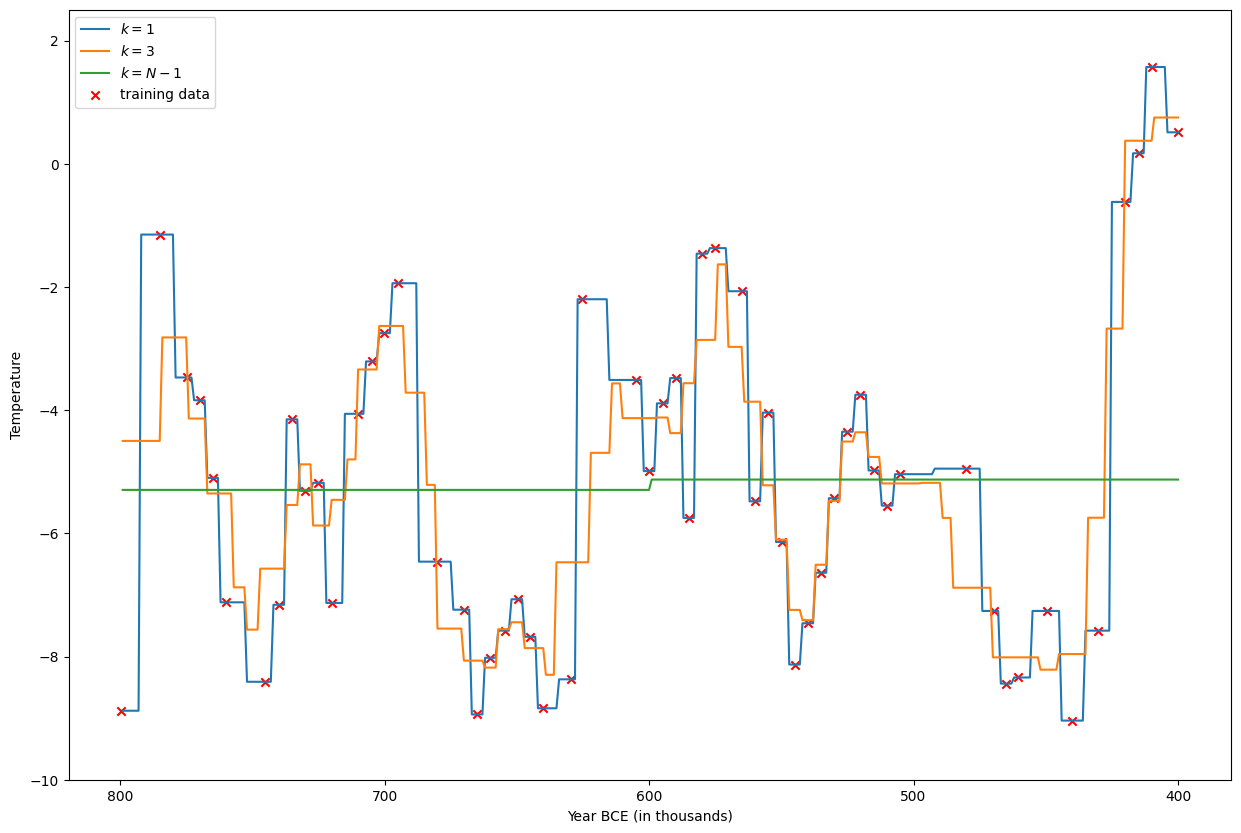
\includegraphics[width=0.8\textwidth]{img_output/p1.1a.png}
            \caption*{\textcolor{blue}{Figure 1.1: Regression lines for different values of $k$}}
            \label{fig:q1.1}
        \end{figure}
        For $k=1$ (blue), the regression line goes exactly through every point in the training set. This makes sense as $k=1$ is the case when our predictor for $x^*$ is the value of $y_n$ corresponding to the $x_n$ that is closest to $x^*$. Thus, for each point $x_n$ in our training set, when we run our regression on $x_n$, we will definitely get $y_n$. We also see around the value $x_n$ in our training set, the regression line is horizontal; this is because points close to $x_n$ just use $y_n$ as their prediction.
        \newline \newline
        For $k=3$ (orange), we see something similar to the $k=1$ case, except it does not hit the extreme points. This is because when $k=3$, we \textit{average} the $y$ values of the nearest 3 data points, not just 1. Thus, an extreme point is not as able to ``pull'' the regression line towards itself; it is balanced by the other 2 points.
        \newline \newline
        For $k=N-1$ (green), we see an almost perfectly horizontal line. It is helpful to think about $k=N$ in explaining this case. For $k=N$, we would see a perfectly horizontal line. This is because our prediction for any new point would just be the average of all data points in the training set. Now, let's consider $k=N-1$. This is the case when our prediction is the average of \textit{all but} the data point in our training set that is \textit{furthest} from the current value of $x_n$ being used for prediction. Thus, for $x_n$ up to around 600K BCE, we have a horizontal line: Our prediction excludes the $y$ value corresponding to the rightmost (smallest value BCE) value of $x$. And for $x_n$ greater than around this 600K BCE cutoff, we again have a horizontal line, but this time it is slightly higher than previously: Our prediction now excludes the $y$ value corresponding to the leftmost (largest value BCE) value of $x$, and includes the right most value of $x$. Note that the leftmost $y$ value is much smaller than the rightmost $y$ value, and this is what causes the upwards shift in the horizontal line.
        \item[(b)] The MSEs are listed below in Table 1.1:
        \begin{table}[H]
            \centering
            \renewcommand{\arraystretch}{1.3} % Increases row height for better readability
            \arrayrulecolor{blue} % Changes the border color to blue
            \begin{tabular}{|c|c|}
                \hline
                \textbf{\textcolor{blue}{k}} & \textbf{\textcolor{blue}{MSE}} \\
                \hline
                \textcolor{blue}{1}  & \textcolor{blue}{1.7406} \\ 
                \textcolor{blue}{3}  & \textcolor{blue}{3.8908} \\ 
                \textcolor{blue}{$N-1$} & \textcolor{blue}{9.5286} \\ 
                \hline
            \end{tabular}
            \caption*{\textcolor{blue}{Table 1.1: MSE values for different values of $k$}}
            \label{tab:mse_k}
        \end{table}
        \vspace{-0.5em}
        The lowest MSE is achieved when $k=1$. In words, our best (in MSE terms) predictor for a new value $x=x^*$ is the value $y_n$ corresponding to the $x_n$ closes to $x^*$. This seems fair for the given dataset, as there are a lot of ``jumps'' within the data, and so a larger value of $k$ would involve averaging over more regions and therefore increasing bias.
    \end{enumerate}
    \item[2.]
    \begin{enumerate}
        \item[(a)] A plot of the model for values $\tau = 1,50,2500$ is shown in Figure 1.2 below:
        \begin{figure}[H]
            \centering
            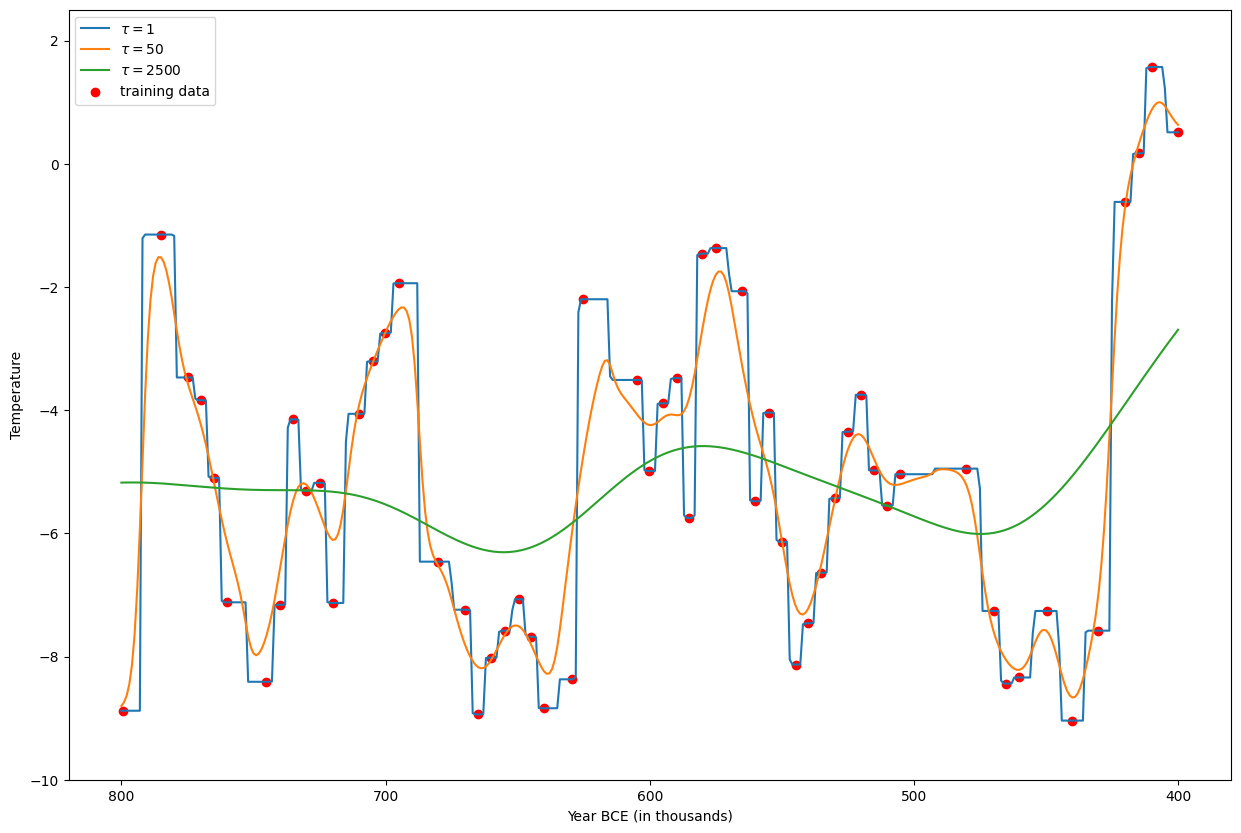
\includegraphics[width=0.7\textwidth]{img_output/p1.2a.png}
            \caption*{\textcolor{blue}{Figure 1.2: Regression lines for different values of $\tau$}}
            \label{fig:q1.2}
        \end{figure}
        For $\tau=1$ (blue), the regression line goes through every training data point. This makes sense, as when $x^*=x_n$ (where $x_n$ is a point in the training set) we have $K_\tau (x_n,x^*) = K_\tau (x_n,x_n) = 1$, and hence $f_\tau (x^*) = f_\tau (x_n) = y_n$. Moreover, for all other $x^*$ such that $|x^* - x_n| > 2$, we have that $K(x_n,x^*) < 0.05$, and so the contribution of that $y_n$ is negligible. Most of the intervals between $x_n$ values in the training set are around 5, so the corresponding kernel is tiny.
        \newline \newline
        For $\tau=50$ (orange), the kernel is more ``forgiving,'' in the sense that $K$ may still be sizable for larger $|x^* - x_n|$. So the kernel function does not penalize as harshly when a new value of $x^*$ is further from an existing training point $x_n$. This gives us the slightly smoother regression line.
        \newline \newline 
        For $\tau=2500$ (green), the process explained in the $\tau=50$ case is taken to the extreme, and a very wide range of $x_n$ values are used in predicting the value of $y^*$. This leads to a lot more smoothing, as observed.
        \item[(b)] The desired expression is
        \begin{align*}
            \text{MSE}_\text{test}(f_\tau) &= \frac{1}{M} \sum_{m=1}^M \left\{ f_\tau (x_m') - y_m' \right\}^2 \\
            \therefore \quad \Aboxed{ \text{MSE}_\text{test}(f_\tau) &= \frac{1}{M} \sum_{m=1}^M \left\{ \frac{\sum_n K_\tau (x_n, x_m')) y_n}{\sum_n K_\tau (x_n,x_m')}-y_m' \right\}^2 }
        \end{align*}
        \item[(c)] The MSE corresponding to each value of $\tau$ is shown in Table 1.2 below:
        \begin{table}[H]
            \centering
            \renewcommand{\arraystretch}{1.3} % Increases row height for better readability
            \arrayrulecolor{blue} % Changes the border color to blue
            \begin{tabular}{|c|c|}
                \hline
                \textcolor{blue}{$\bm{\tau}$} & \textbf{\textcolor{blue}{MSE}} \\
                \hline
                \textcolor{blue}{1}  & \textcolor{blue}{1.9473} \\ 
                \textcolor{blue}{50}  & \textcolor{blue}{1.8583} \\ 
                \textcolor{blue}{2500} & \textcolor{blue}{8.3339} \\ 
                \hline
            \end{tabular}
            \caption*{\textcolor{blue}{Table 1.2: MSE values for different values of $\tau$}}
            \label{tab:mse_tau}
        \end{table}
        The model that yields the lowest MSE is the one corresponding to $\tau=50$. Conceptually, this represents a balance between fitting the data well whilst also capturing the true underlying pattern.
        \newline \newline
        Choosing $\tau$ based on $\mathcal{D}_\text{train}$ rather than $\mathcal{D}_\text{test}$ would result in overfitting: If we train over the training data set and then validate on the train set again, we are choosing a value of $\tau$ that encourages our model to conform to the exact variation in our train dataset instead of finding generalizable trends.
        \item[(d)] The time and space complexities of each method are detailed in Table 1.3 below:
        \begin{table}[H]
            \centering
            \renewcommand{\arraystretch}{1.3} % Adjust row height
            \arrayrulecolor{blue} % Change table border color to blue
            \begin{tabular}{|c|c|c|}
                \hline
                \textbf{\textcolor{blue}{Method}} & \textbf{\textcolor{blue}{Time}} & \textbf{\textcolor{blue}{Space}} \\ 
                \hline
                \textcolor{blue}{kNN} & \textcolor{blue}{$O(N\log N)$} & \textcolor{blue}{$O(N)$} \\ 
                \textcolor{blue}{kernelized} & \textcolor{blue}{$O(N)$} & \textcolor{blue}{$O(N)$} \\ 
                \hline
            \end{tabular}
            \caption*{\textcolor{blue}{Table 1.3: Time and space complexities of kNN and kernelized regression}}
            \label{tab:knn_kernel}
        \end{table}
        For kNN, we need $O(N)$ space to store the training data, as all of these points are required to make each new prediction. The runtime is $O(N\log N)$. This is achieved using merge sort: Sort the train set in order of distance from $x^*$, and choose the first $k$ elements of that list.
        \newline \newline
        For kernelized regression, we again need $O(N)$ space to store the train set, as all of these points are used in making a new prediction. The runtime is $O(N)$: We just need to apply $K_\tau$ to each $x_n$ in our train set.
        \item[(e)] Consider 2 arbitrary points $x_1,x_2$ in our train set. Suppose we are trying to predict the $y^*$ value of some new point, $x^*$. We first look at the following ratio:
        \begin{align*}
            \frac{K_\tau(x_1,x^*)}{K_\tau(x_2,x^*)} &= \frac{\exp \left({\frac{-(x_1-x^*)^2}{\tau}}\right)}{\exp \left({\frac{-(x_2-x^*)^2}{\tau}}\right)} = \exp \left\{ \frac{1}{\tau} \left\{ (x_2-x^*)^2 - (x_1-x^*)^2 \right\} \right\} \\
            \therefore \quad \lim_{\tau \to 0} \frac{K_\tau(x_1,x^*)}{K_\tau(x_2,x^*)} &= \begin{cases} 
                                    0, & \text{if } |x_1-x^*| > |x_2-x^*| \\
                                    1, & \text{if } |x_1-x^*| = |x_2-x^*| \\
                                    \infty, & \text{if } |x_1-x^*| < |x_2-x^*|
                                \end{cases}
        \end{align*}
        Let the set $\mathcal{K} = \arg\min\limits_{n} \left\{ (x_n-x^*)^2 \right\}$. Since $(x_k-x^*)^2$ and hence $K(x_k,x^*)$ is the same for all $k \in \mathcal{K}$, then we can arbitrarily pick a $k \in \mathcal{K}$:
        \begin{align*}
            f_\tau(x^*) &= \frac{\sum_n K_\tau(x_n, x^*)y_n}{\sum_nK_\tau(x_n, x^*)} \\
            &= \frac{\sum_n \frac{K_\tau(x_n,x^*)}{K_\tau(x_k,x^*)}y_n}{\sum_n \frac{K_\tau(x_n,x^*)}{K_\tau(x_k,x^*)}} \\
            \therefore \quad \Aboxed{ \lim_{\tau \to 0} f_\tau(x^*) &= \frac{1}{|\mathcal{K}|}\sum_{k \in \mathcal{K}}y_k }
        \end{align*}
        as $\lim_{\tau \to 0} \frac{K_\tau(x_n,x^*)}{K_\tau(x_k,x^*)} = 0$ for all $n \notin \mathcal{K}$ and 1 for all $n \in \mathcal{K}$.
    \end{enumerate}
\end{enumerate}

\end{solution}


%%%%%%%%%%%%%%%%%%%%%%%%%%%%%%%%%%%%%%%%%%%%%
% Problem 2
%%%%%%%%%%%%%%%%%%%%%%%%%%%%%%%%%%%%%%%%%%%%%
\newpage
\begin{problem}[Deriving Linear Regression, 20pts]

We now seek to model the temperatures with a parametric method: linear regression. Before we implement anything, let's revisit the mathematical formulation of linear regression.  Specifically, the solution for the least squares linear regression  ``looks'' kind of like a ratio of covariance and
variance terms.  In this problem, we will make that connection more
explicit. \\

\noindent Suppose we have some 2-D data where each observation has the form $(x, y)$ and is independent and identically distributed according  $x \sim p(x)$, $y \sim p(y|x)$. We will consider the process of fitting these data from this distribution with the best linear model
possible, that is a linear model of the form $\hat{y} = wx$ that
minimizes the expected squared loss $E_{x,y}[ ( y - \hat{y} )^2
    ]$.\\

\noindent Note: The notation $E_{x, y}$ indicates an
expectation taken over the joint distribution $p(x,y)$. This essentially just means to treat $x$ and $y$ as random.  

\begin{enumerate}

  \item Derive an expression for the optimal $w$, that is, the $w$
        that minimizes the expected squared loss above.  You should leave
        your answer in terms of moments of the distribution, e.g. terms
        like $E_x[x]$, $E_x[x^2]$, $E_y[y]$, $E_y[y^2]$, $E_{x,y}[xy]$
        etc.

  \item Note that while $x, y$ are data that we have access to, $E_{x, y}[yx]$ is a theoretical constant. Keeping in mind the interpretation of expectations as average values, how could you use observed data $\{(x_n,y_n)\}_{n=1}^N$ to estimate $E_{x, y}[yx]$ and $E_x[x^2]$?

  \item In general, moment terms like $E_{x, y}[yx]$, $E_{x, y}[x^2]$,
        $E_{x, y}[yx^3]$, $E_{x, y}[\frac{x}{y}]$, etc. can easily be
        estimated from the data (like you did above).  If you substitute in
        these empirical moments, how does your expression for the optimal
        $w^*$ in this problem compare with the optimal $\bm{\hat w}$ from Problem 4.3 of HW0?

  \item Many common probabilistic linear regression models assume that
        variables $x$ and $y$ are jointly Gaussian.  Did any of your above
        derivations rely on the assumption that $x$ and $y$ are jointly
        Gaussian?  Why or why not?
\end{enumerate}
\end{problem}

\newpage
\begin{solution}

\begin{enumerate}
    \item [1.] Let $\mathcal{L}(w) = \mathbb{E}_{x,y}\left\{ \left(y-\hat{y}\right)^2\right\}$. Expanding out, we get
    \begin{align*}
        \mathcal{L}(w) &= \mathbb{E}_{x,y} \left\{ \left(y-wx\right)^2 \right\} \\
        &= \mathbb{E}_{x,y} \left\{ y^2 - 2wxy + w^2x^2 \right\} \\
        \therefore \quad \mathcal{L}(w) &= \mathbb{E}_y \left\{ y^2 \right\} - 2w \cdot \mathbb{E}_{x,y}\left\{ xy \right\} + w^2 \mathbb{E}_{x}\left\{ x^2\right\} \tag*{(2.1.1)}
    \end{align*}
    The goal is to minimize $\mathcal{L}(w)$. Take the first derivative of (2.1.1) w.r.t. $w$ and set it to 0 to find the optimal $w^*$:
    \begin{align*}
        \frac{d\mathcal{L}(w)}{dw} = -2\mathbb{E}_{x,y}\left\{xy\right\} + 2w^*\mathbb{E}_{x}\left\{x^2\right\} &= 0 \\
        \therefore \quad \Aboxed{ w^* &= \frac{\mathbb{E}_{x,y}\{xy\} }{\mathbb{E}_x\left\{x^2\right\} } } \tag*{(2.1.2)}
    \end{align*}

    \item[2.] We will use the Method of Moments to arrive at the following estimates:
    \begin{align*}
        \Aboxed{ \widehat{ \mathbb{E}_{x,y}[xy] } &= \frac{1}{N} \sum_{n=1}^N x_ny_n } \tag*{(2.2.1)}
    \end{align*}
    \begin{align*}
        \Aboxed{ \widehat{ \mathbb{E}_{x}\left[x^2\right] } &= \frac{1}{N} \sum_{n=1}^N x_n^2 } \tag*{(2.2.2)}
    \end{align*}

    \item[3.] Our estimate here in terms of the empirical moments is
    \begin{align*}
        w^* &= \frac{\sum_{n=1}^N x_ny_n}{\sum_{n=1}^N x_n^2} \tag*{(2.3.1)}
    \end{align*}
    Next, we derive an expression for $w^*$ using (4.3) from HW0:
    \begin{align*}
        \mathbf{w}^* &= \left(\mathbf{X}^\mathrm{T}\mathbf{X}\right)^{-1}\mathbf{X}^\mathrm{T}\mathbf{y} 
    \end{align*}
    where $\mathbf{X} = \begin{bmatrix}
        x_1 \\ x_2 \\ \vdots \\ x_n
    \end{bmatrix}$ and $\mathbf{y} = \begin{bmatrix}
        y_1 \\ y_2 \\ \vdots \\ y_n
    \end{bmatrix}$. Hence, $\mathbf{w}^*$ is a scalar:
    \begin{align*}
        w^* &= \left\{ \sum_{n=1}^N x_n^2 \right\}^{-1} \sum_{n=1}^{N} x_ny_n = \frac{\sum_{n=1}^N x_ny_n}{\sum_{n=1}^N x_n^2} \tag*{(2.3.2)}
    \end{align*}
    We can see that (2.3.1) and (2.3.2) are both equivalent. So our expression for the optimal $w^*$ is the same when using Method of Moments vs. OLS.

    \item[4.] None of the above derivations rely on the assumption that $x$
and $y$ are jointly Gaussian. This is because our estimate for the optimal $w^*$ depends only on two summary statistics (expectations). Since these statistics are computed directly from the given data---\textit{treating them as fixed values}---the derivation does not impose any assumptions on the underlying data-generating distribution.
\end{enumerate}
\end{solution}

%%%%%%%%%%%%%%%%%%%%%%%%%%%%%%%%%%%%%%%%%%%%%
% Problem 3
%%%%%%%%%%%%%%%%%%%%%%%%%%%%%%%%%%%%%%%%%%%%%
\newpage
\begin{problem}[Basis Regression, 30pts]

 Having reviewed the theory, we now implement some linear regression models for the temperature. If we just directly use the data as given to us, we would only have
    a one dimensional input to our model, the year.  To create a more expressive linear
    model, we will introduce basis functions.

\vspace{1em}

\noindent\emph{Make sure to include all required plots in your PDF.}

\begin{enumerate}
  \item
        We will first implement the four basis regressions below. (The first basis has been implemented for you in the notebook as an example.) Note that we introduce an addition transform $f$ (already into the provided notebook) to address concerns about numerical instabilities.
        \begin{enumerate}
          \item $\phi_j(x)= f(x)^j$ for $j=1,\ldots, 9$. $f(x) = \frac{x}{1.81 \cdot 10^{2}}.$
          \item $\phi_j(x) = \exp\left\{-\cfrac{(f(x)-\mu_j)^2}{5}\right\}$ for $\mu_j=\frac{j + 7}{8}$ with $j=1,\ldots, 9$. $f(x) = \frac{x}{4.00 \cdot 10^{2}}.$
          \item $\phi_j(x) =  \cos(f(x) / j)$ for $j=1, \ldots, 9$. $f(x) = \frac{x}{1.81}$.
          \item $\phi_j(x) = \cos(f(x) / j)$ for $j=1, \ldots, 49$. $f(x) = \frac{x}{1.81 \cdot 10^{-1}}$. \footnote{For the trigonometric bases (c) and (d), the periodic nature of
                  cosine requires us to transform the data such that the
                  lengthscale is within the periods of each element of our basis.}
        \end{enumerate}

        {\footnotesize * Note: Please make sure to add a bias term for
        all your basis functions above in your implementation of the
        \verb|make_basis|.}

        Let
        $$ \mathbf{\phi}(\mathbf{X}) =
          \begin{bmatrix}
            \mathbf{\phi}(x_1) \\
            \mathbf{\phi}(x_2) \\
            \vdots             \\
            \mathbf{\phi}(x_N) \\
          \end{bmatrix} \in \mathbb{R}^{N\times D}.$$
        You will complete the \verb|make_basis| function which must return
        $\phi(\mathbf{X})$ for each part
        (a) - (d). You do NOT need to submit this
        code in your \LaTeX writeup.

        Then, create a plot of the fitted
        regression line for each basis against a scatter plot
        of the training data. Boilerplate plotting code is provided in the
        notebook---you will only need to finish up a part of it.
        \textbf{All you need to include
          in your writeup for this part are these four plots.}

        \item
          Now we have trained each of our basis regressions. For each basis
          regression, compute the MSE on the test set.  Discuss: do any of the
          bases seem to overfit?  Underfit?  Why?


    \item Briefly describe what purpose the transforms $f$ serve: why are they helpful?

    \item As in Problem 1, describe the space and time complexity of linear regression.  How does what is stored to compute predictions change with the size of the training set $N$ and the number of features $D$?  How does the computation needed to compute the prediction for a new input depend on the size of the training set $N$?  How do these complexities compare to those of the kNN and kernelized regressor?

    \item Briefly compare and constrast the different regressors: kNN,
          kernelized regression, and linear regression (with bases).  Are some
          regressions clearly worse than others?  Is there one best
          regression?  How would you use the fact that you have these multiple
          regression functions?

  \end{enumerate}
  Note:
  Recall that we are using a
  different set of inputs $\mathbf{X}$ for each basis (a)-(d).
  Although it may seem as though this prevents us from being able
  to directly compare the MSE since we are using different data,
  each transformation can be considered as being a part of our model.
  Contrast this with transformations (such as standardization) that cause the variance of the target $\mathbf{y}$ to be different; in these cases the
  MSE can no longer be directly compared.
\end{problem}

\newpage 
\begin{solution}

\begin{enumerate}
    \item [1.] The plots are included in Figure 3.1 below.
    \vspace{-1em}
    \begin{figure}[H]
    \centering
    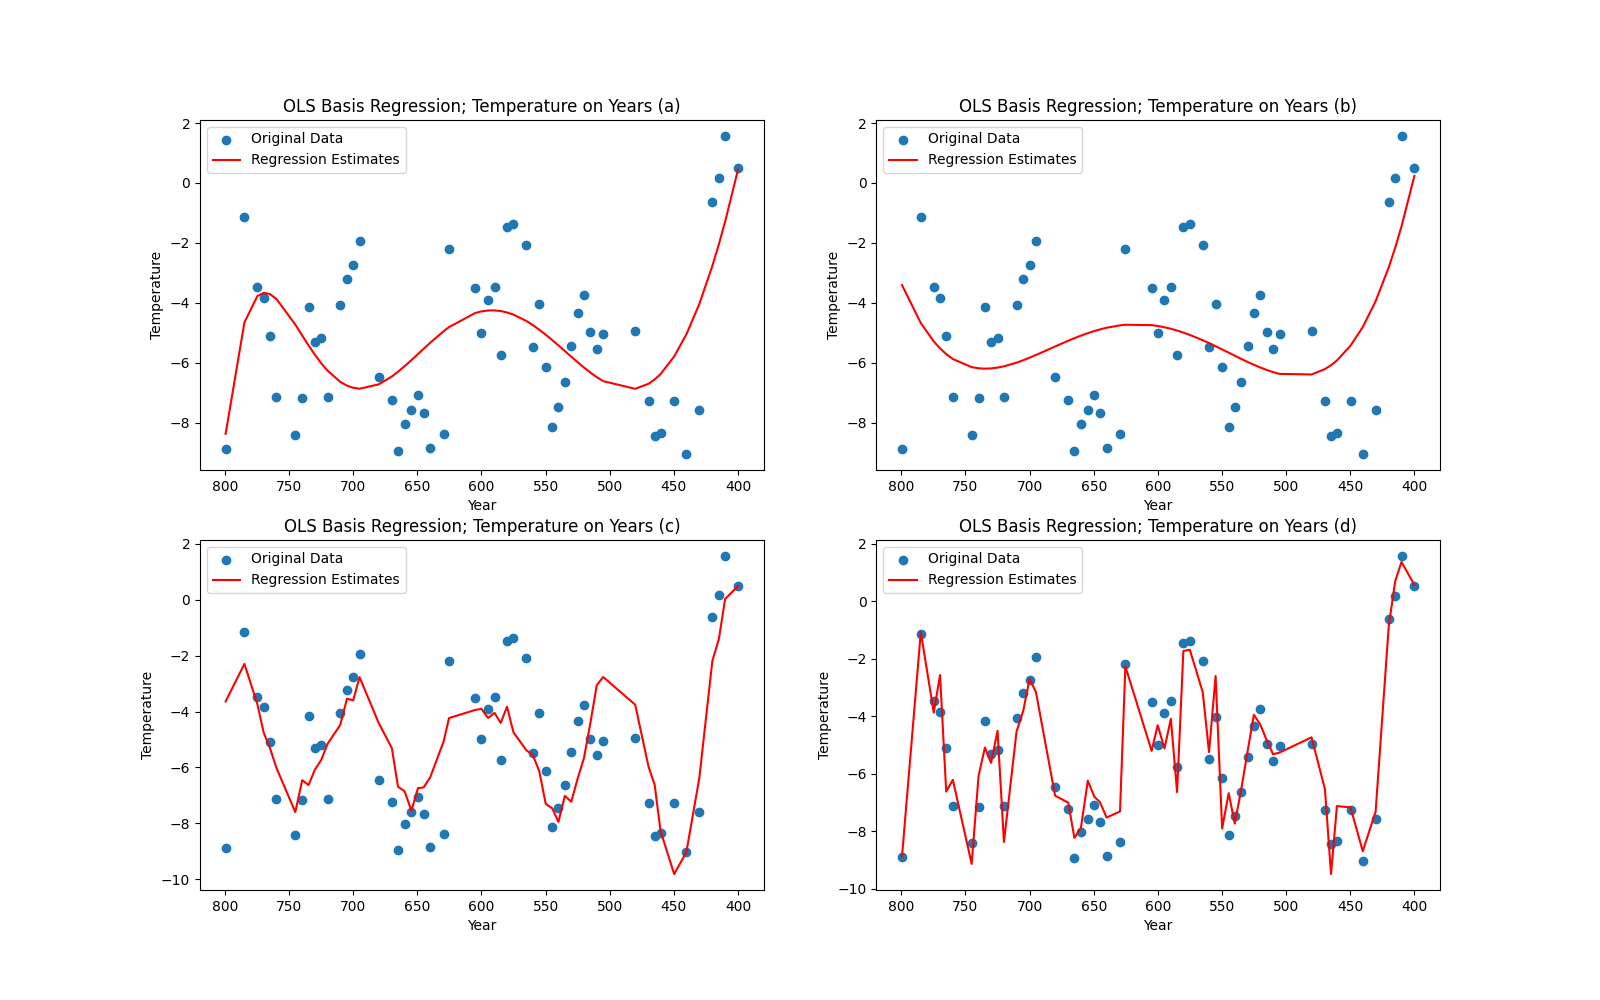
\includegraphics[width=0.98\textwidth]{img_output/p3.1.png}
    \caption*{\textcolor{blue}{Figure 3.1: Fitted regression lines for different bases}}
    \label{fig:q3.1}
    \end{figure}
    \item[2.] MSEs are listed in Figure 3.2 below:
    \begin{table}[H]
        \centering
        \arrayrulecolor{blue}
        \renewcommand{\arraystretch}{1.2} % Adjust row height for readability
    
        \begin{tabular}{|c|c|}
            \hline
            \textbf{\textcolor{blue}{Basis}} & \textbf{\textcolor{blue}{MSE}} \\ 
            \hline
            \textcolor{blue}{a} & \textcolor{blue}{7.9558} \\ 
            \textcolor{blue}{b} & \textcolor{blue}{8.7081} \\ 
            \textcolor{blue}{c} & \textcolor{blue}{5.9670} \\ 
            \textcolor{blue}{d} & \textcolor{blue}{58.9471} \\ 
            \hline
        \end{tabular}
        
        \caption*{\textcolor{blue}{Figure 3.2: MSE for each basis}}
        \label{tab:mse_comparison}
    \end{table}
    Basis d definitely overfits. We observe a very high test MSE relative to other bases, even though the regression line fits the training set the best out of all the bases. This is to be expected: Basis d uses 49 basis functions, so including the intercept, this gives us 50 ``dimensions.'' We only have 57 data points. In the extreme case where we would have 57 dimensions in our model. In this case, we would have one dimension per data point, and our model would predict every point in the training set \textit{exactly}, with each predictor just corresponding to a data point. The model would thus not generalize at all. 50 dimensions is still very close to 57 and this explains the high degree of overfitting for basis d.
    \newline \newline
    Bases a and b appears to underfit: They have higher MSEs than basis c on the test set, yet both are smoother than basis c when fitted on the train set.
    \item[3.] The purpose of the transforms $f$ is to prevent numerical instabilities. Each $f$ scales $x$ by some constant factor to ensure that the inputs to the basis functions are within a reasonable range. This is particularly important for e.g., basis a, which is a polynomial function, and if $x$ is too large, then $x^j$ could grow very large and cause overflow or precision errors. This will also help prevent large inputs from dominating computation. The footnote explains how the periodic nature of cosine in bases c and d requires us to transform the data in order to prevent very rapid oscillations (which could in turn lead to overfitting).
    \newline \newline
    These transformations also make the basis functions more readable by abstracting away and allowing us to focus on the overall structure or form of the basis function.
    \item[4.] We extend Table 1.3 with the time and space complexities for linear regression in Table 3.4:
        \begin{table}[H]
            \centering
            \renewcommand{\arraystretch}{1.3} % Adjust row height
            \arrayrulecolor{blue} % Change table border color to blue
            \begin{tabular}{|c|c|c|}
                \hline
                \textbf{\textcolor{blue}{Method}} & \textbf{\textcolor{blue}{Time}} & \textbf{\textcolor{blue}{Space}} \\ 
                \hline
                \textcolor{blue}{kNN} & \textcolor{blue}{$O(N\log N)$} & \textcolor{blue}{$O(N)$} \\ 
                \textcolor{blue}{kernelized} & \textcolor{blue}{$O(N)$} & \textcolor{blue}{$O(N)$} \\ 
                \textcolor{blue}{linear regression} & \textcolor{blue}{$O(D)$} & \textcolor{blue}{$O(D)$} \\ 
                \hline
            \end{tabular}
            \caption*{\textcolor{blue}{Table 3.4: Time and space complexities for different regressions}}
            \label{tab:knn_kernel}
        \end{table}
    \textit{Given} a fitted model, predicting the response of a new data point $\mathbf{x^*}$ takes $O(D)$: We just have to take the dot product $\mathbf{\hat{w}}^\mathrm{T}\mathbf{x^*}$. The dimension of each of $\mathbf{\hat{w}}, \mathbf{x^*}$ is $D$. Thus, prediction takes $O(D)$. Moreover, the only data we need to store are these two vectors, which is again $O(D)$. However, when actually fitting the model (which we will consider to be preprocessing), we need $O\left(N^2D + D^3\right)$ which reduces to $O\left(N^2D\right)$ since in practice, $N > D$. The space complexity is correspondingly $O\left(ND +D^2\right)$ which reduces to $O\left(ND\right)$.
    \newline \newline
    Looking at Table 3.4, it becomes clear that linear regression is superior, \textit{when judged in terms of time and space complexity}, especially since $N \gg D$ in practice.
    \item[5.] It appears that kNN (when using the optimal value of $k$) gave the lowest MSE out of all 3 regressions, with an MSE of around 1.74. However, this is not much better than kernelized, where the best MSE (out of the 3 values of $\tau$ we simulated) was around 1.86. Moreover, both regressions take the same complexity, but kernelized has a faster runtime (see Table 3.4). Thus, one could reasonably argue that kernelized is better than kNN on balance. 
    \newline \newline
    The best MSE achieved in basis regression was for basis c, with an MSE of around 5.97. This is substantially larger than kNN and kernelized. However, linear regression brings the benefit of much lower time and space complexity, especially for large $N$. Additionally, linear regression is more likely to generalize for data points beyond the dataset range. This is because it forms an interpretable relationship between response and predictors, building the vector of weights. Linear regression uses the training set to ``learn,'' then applies this model to new inputs. By contrast, kNN would just output the average of the $k$ largest $y_n$ in the train set, no matter how large the new input gets (i.e., it would not scale). Kernelized would similarly be a poor predictor on large new inputs beyond the range of the train set: If $x^*$ is large, then the exponent in the given kernel function will be very negative and so the kernel will go to 0, and so our prediction will collapse.
    \newline \newline
    A final caveat is that we have only tested out these regressions on a single train and test dataset. If we wanted to achieve a more comprehensive understanding of which regressions are optimal in certain cases, then we would have to run each of these on multiple different datasets.
\end{enumerate}
\end{solution}
%%%%%%%%%%%%%%%%%%%%%%%%%%%%%%%%%%%%%%%%%%%%%
% Problem 4
%%%%%%%%%%%%%%%%%%%%%%%%%%%%%%%%%%%%%%%%%%%%%
\begin{problem}[Probablistic Regression and Regularization, 30pts]

Finally, we will preview Bayesian regression and explore its connection to regularization for linear models. Then, we will fit a regularized model to the temperature data. Although the content is related, you do not need to know the material from the lectures on frequentist model selection and Bayesian model selection to solve this problem.  \\

\noindent Recall that the probabilistic version of linear regression states that 
\[y_n = \boldw^\top\boldx_n + \epsilon_n, \quad \epsilon_n \sim \mathcal{N}(0, \sigma^2)\]
In Bayesian regression, we impose a prior $p(\boldw)$ on the weights and  fit the weights $\boldw$ through maximizing the posterior likelihood
\[p(\boldw | \boldX, \boldy) = \frac{p(\bold y | \boldw, \boldX)p(\boldw)}{p(\boldy | \boldX)}\]
Note: since we maximize with respect to $\boldw$, it suffices to just maximize the numerator.

\begin{enumerate}
    \item Suppose $\boldw \sim \mathcal{N}(\mathbf{0},\frac{\sigma^2}{\lambda}\boldI)$. Show that maximizing the posterior likelihood is equivalent to minimizing 
    \[\mathcal{L}_{ridge}(\boldw) = \frac{1}{2}||\boldy -\bold X\boldw||_2^2 + \frac{\lambda}{2}||\boldw||_2^2.\] 
    Note that minimizing $\mathcal{L}_{ridge}(\boldw)$ is exactly what ridge regression does.
    
    Hint: You don't need to solve for the maximizer/minimizer to show that the optimization problems are equivalent.
    
    \item Solve for the value of $\boldw$ that minimizes $\mathcal L_{ridge}(\boldw)$.

    \item The Laplace distribution has the PDF
   \[L(a,b) =\frac{1}{2b} \exp\left(-\frac{|x - a|}{b}\right)\]
Show that if all $w_d \sim L\left(0,\frac{2\sigma^2}{\lambda}\right)$, maximizing the posterior likelihood is equivalent to minimizing 
\[\mathcal{L}_{lasso}(\boldw) = \frac{1}{2}||\boldy -\bold X\boldw||_2^2  + \frac{\lambda}{2}||\boldw||_1.\] 
Note that minimizing $\mathcal{L}_{lasso}(\boldw)$ is exactly what LASSO regression does.

    \item Why is there no general closed form for the LASSO estimator, i.e. the value of $\boldw$ that minimizes $\mathcal{L}_{ridge}(\boldw)$?

    \item Since there is no general closed form for LASSO, we use numerical methods for estimating $\boldw$. One approach is to use \textit{coordinate descent}, which works as follows: 
    \begin{enumerate}
        \item Initialize $\boldw=\boldw_0$.
        \item For each $d=1, \ldots, D$ do the following 2 steps consecutively:
        \begin{enumerate}
            \item Compute $\rho_d = \tilde{\boldx}_d^\top(\boldy - (\boldX \boldw - w_d \tilde{\boldx}_d))$. We define $\tilde{\boldx}_d$ as the $d$-th column of $\boldX$.

            \item If $d=1$, set $w_1 = \frac{\rho_1}{||\tilde{\boldx}_1||^2_2}$. Otherwise if $d\ne 1$, compute $w_d = \frac{\text{sign}(\rho_d)\max\left\{|\rho_d|-\frac{\lambda}{2}, 0\right\}}{||\tilde{\boldx}_d||^2_2}$.
        \end{enumerate}
        \item Repeat step (b) until convergence or the maximum number of iterations is reached.
    \end{enumerate} 

    Implement the \texttt{find\_lasso\_weights} function according to the above algorithm, letting $\boldw_0$ be a vector of ones and the max number of iterations be 5000. Then, fit models with $\lambda=1, 10$ to basis (d) from Problem 3, plot the predictions, and compute the MSE's. You will need to do some preprocessing, but a completed helper function for this is already provided. How do the graphs and errors compare to those for the unregularized basis (d) model? 


\end{enumerate}

\end{problem}

\newpage
\begin{solution}

\begin{enumerate}
    \item [1.] We have that
    \begin{align*}
        \mathbf{y} &= \begin{bmatrix}
            y_1 \\ y_2 \\ \vdots \\ y_n
        \end{bmatrix} = \begin{bmatrix}
            \mathbf{w}^\mathrm{T}\mathbf{x}_1 + \epsilon_1 \\
            \mathbf{w}^\mathrm{T}\mathbf{x}_2 + \epsilon_2 \\
            \vdots \\
            \mathbf{w}^\mathrm{T}\mathbf{x}_N + \epsilon_N
        \end{bmatrix} = \mathbf{X}\mathbf{w} + \mathbf{\epsilon}
    \end{align*}
    Since $\mathbf{\epsilon} \sim \mathcal{N}\left(\mathbf{0}, \sigma^2\mathbf{I}\right)$, and noting that we are \textit{conditioning on the data} (and therefore treating $\mathbf{X}\mathbf{w}$ as a constant), we have
    \begin{align*}
        p(\mathbf{y} | \mathbf{w}, \mathbf{X}) &= \mathcal{N}\left(\mathbf{y} |  \mathbf{X}\mathbf{w}, \sigma^2\mathbf{I}\right) \\
        &= \frac{1}{(2\pi)^{N/2}}\frac{1}{\lvert \sigma^2\mathbf{I} \rvert^{1/2}} \exp \left\{ -\frac{1}{2}\left(\mathbf{y} - \mathbf{X}\mathbf{w}\right)^\mathrm{T}{\left(\sigma^2\mathbf{I}\right)}^{-1} \left( \mathbf{y} - \mathbf{X}\mathbf{w} \right) \right\} \\
        &\propto \exp \left\{ -\frac{1}{2\sigma^2}\left(\mathbf{y} - \mathbf{X}\mathbf{w}\right)^\mathrm{T}\left( \mathbf{y} - \mathbf{X}\mathbf{w} \right) \right\} \\
        \therefore \quad p(\mathbf{y} | \mathbf{w}, \mathbf{X}) &\propto \exp \left\{ -\frac{1}{2\sigma^2}\left\lVert \mathbf{y} - \mathbf{X}\mathbf{w}  \right\rVert_2^2 \right\} \tag*{(4.1.1)}
    \end{align*}
    Also, we are told to assume that $\mathbf{w} \sim \mathcal{N}\left( \mathbf{0}, \frac{\sigma^2}{\lambda}\mathbf{I}\right)$, we have that
    \begin{align*}
        p(\mathbf{w}) &= \mathcal{N}\left( \mathbf{0}, \frac{\sigma^2}{\lambda}\mathbf{I}\right) \\
        &= \frac{1}{(2\pi)^{N/2}}\frac{1}{\left\lvert \frac{\sigma^2}{\lambda}\mathbf{I} \right\rvert^{1/2}} \exp \left\{ -\frac{1}{2}\left( \mathbf{w} - \mathbf{0} \right)^\mathrm{T}{\left(\frac{\sigma^2}{\lambda}\mathbf{I}\right)}^{-1} \left( \mathbf{w} - \mathbf{0} \right) \right\} \\
        &\propto \exp \left\{ -\frac{\lambda}{2\sigma^2}\mathbf{w}^\mathrm{T}\mathbf{w} \right\} \\
        \therefore \quad p(\mathbf{w}) &\propto \exp \left\{ -\frac{\lambda}{2\sigma^2}\lVert \mathbf{w} \rVert_2^2 \right\} \tag*{(4.1.2)}
    \end{align*}
    Combining (4.1.1) and (4.1.2), and noting that $p(\mathbf{y}|\mathbf{X})$ is independent of $\mathbf{w}$, we have
    \begin{align*}
        p(\mathbf{w}|\mathbf{X},\mathbf{y}) &\propto p(\mathbf{y}|\mathbf{w},\mathbf{X})p(\mathbf{w}) \\
        &\propto \exp \left\{ -\frac{1}{2\sigma^2}\left\lVert \mathbf{y} - \mathbf{X}\mathbf{w}  \right\rVert_2^2 \right\} \exp \left\{ -\frac{\lambda}{2\sigma^2}\lVert \mathbf{w} \rVert_2^2 \right\} \\
        \therefore \quad p(\mathbf{w}|\mathbf{X},\mathbf{y}) &\propto \exp \left\{ -\frac{1}{2\sigma^2}\left\lVert \mathbf{y} - \mathbf{X}\mathbf{w}  \right\rVert_2^2 - \frac{\lambda}{2\sigma^2}\lVert \mathbf{w} \rVert_2^2 \right\} \tag*{(4.1.3)}
    \end{align*}
    (4.1.3) shows us that the posterior likelihood $p(\mathbf{w}|\mathbf{X},\mathbf{y})$ is maximized iff the exponent is maximized, which occurs iff $\frac{1}{2\sigma^2}\left\lVert \mathbf{y} - \mathbf{X}\mathbf{w}  \right\rVert_2^2 + \frac{\lambda}{2\sigma^2}\lVert \mathbf{w} \rVert_2^2$ is minimized. Since $\sigma^2$ is a constant, then maximizing the posterior likelihood is equivalent to minimizing
    \begin{align*}
        \mathcal{L}_\text{ridge}(\mathbf{w}) &= \frac{1}{2}\left\lVert \mathbf{y} - \mathbf{X}\mathbf{w}  \right\rVert_2^2 + \frac{\lambda}{2}\lVert \mathbf{w} \rVert_2^2 \tag*{(4.1.4)}
    \end{align*}
    \item[2.] We solve for the value of $\mathbf{w}$ that minimizes (4.1.4) by setting the first derivative to 0. Before we do so, it is helpful to rewrite (4.1.4) as follows:
    \begin{align*}
        \mathcal{L}_\text{ridge}(\mathbf{w}) &= \frac{1}{2}\left(\mathbf{y} - \mathbf{X}\mathbf{w}\right)^\mathrm{T}\left( \mathbf{y} - \mathbf{X}\mathbf{w} \right) + \frac{\lambda}{2} \mathbf{w}^\mathrm{T}\mathbf{w} \tag*{(4.2.1)}
    \end{align*}
    Using standard results, we set the first derivative of (4.2.1) to 0:
    \begin{align*}
        \frac{\partial \mathcal{L}_\text{ridge}(\mathbf{w})}{\partial \mathbf{w}} = \left(-\mathbf{X}^\mathrm{T}\right)\left(\mathbf{y}-\mathbf{X}\mathbf{w^*}\right) + \mathbf{w^*} &= 0 \\
        \therefore \quad \left(\mathbf{X}^\mathrm{T}\mathbf{X} + \lambda\mathbf{I}\right)\mathbf{w^*} &= \mathbf{X}^\mathrm{T}\mathbf{y} \\
        \therefore \quad \Aboxed{ \mathbf{w^*} &= \left(\mathbf{X}^\mathrm{T}\mathbf{X} + \lambda\mathbf{I} \right)^{-1} \mathbf{X}^\mathrm{T}\mathbf{y} } \tag*{(4.2.2)}
    \end{align*}
    \item[3.] Note that we still have
    \begin{align*}
        p(\mathbf{y} | \mathbf{w}, \mathbf{X}) &\propto \exp \left\{ -\frac{1}{2\sigma^2}\left\lVert \mathbf{y} - \mathbf{X}\mathbf{w}  \right\rVert_2^2 \right\} \tag*{(4.3.1)}
    \end{align*}
    as in (4.1.1).

    However, under the assumption that the elements of $\mathbf{w}$ are i.i.d. per this (\url{https://edstem.org/us/courses/74317/discussion/6163769}) Ed post, the prior on $\mathbf{w}$ is now
    \begin{align*}
        p(\mathbf{w}) &= \prod_{d=1}^D \frac{1}{2\left(2\sigma^2/\lambda\right)}\exp \left\{ -\frac{\left\lvert w_d - 0 \right\rvert}{2\sigma^2/\lambda} \right\} \\
        &\propto \exp \left\{ -\frac{\sum_{d=1}^D \lvert w_d \rvert}{2\sigma^2/\lambda} \right\} \\
        \therefore \quad p(\mathbf{w}) &\propto \exp \left\{ -\frac{\lambda \lVert \mathbf{w} \rVert_1}{2\sigma^2} \right\} \tag*{(4.3.2)}
    \end{align*}
    Taking a similar approach as in part (1), we have
    \begin{align*}
        p(\mathbf{w}|\mathbf{X},\mathbf{y}) &\propto p(\mathbf{y}|\mathbf{w},\mathbf{X})p(\mathbf{w}) \\
        &\propto \exp \left\{ -\frac{1}{2\sigma^2}\left\lVert \mathbf{y} - \mathbf{X}\mathbf{w}  \right\rVert_2^2 \right\} \exp \left\{ -\frac{\lambda \lVert \mathbf{w} \rVert_1}{2\sigma^2} \right\} \\
        \therefore \quad p(\mathbf{w}|\mathbf{X},\mathbf{y}) &\propto \exp \left\{ -\frac{1}{2\sigma^2}\left\lVert \mathbf{y} - \mathbf{X}\mathbf{w}  \right\rVert_2^2 - \frac{\lambda \lVert \mathbf{w} \rVert_1}{2\sigma^2} \right\} \tag*{(4.3.3)}
    \end{align*}
    and thus maximizing the posterior likelihood is equivalent to minimizing the negative of the exponent in (4.3.3), which is equivalent to minimizing
    \begin{align*}
        \mathcal{L}_\text{lasso}(\mathbf{w}) &= \frac{1}{2}\left\lVert \mathbf{y} - \mathbf{X}\mathbf{w}  \right\rVert_2^2 + \frac{\lambda}{2} \lVert \mathbf{w} \rVert_1 \tag*{(4.3.4)}
    \end{align*}
    \item[4.] There is no general closed-form solution for the LASSO estimator because the L1 norm introduces nondifferentiability at 0. In theory, one could build a piecewise function that accounts for different cases for each entry of $\mathbf{w}$; however, the number of such cases grows exponentially with the number of parameters and is thus infeasible in practice.
    \clearpage
    \item[5.] Figure 4.5 shows a plot of the predictions against the true values for the training set, for $\lambda = 1,10$:
    \begin{figure}[H]
        \centering
        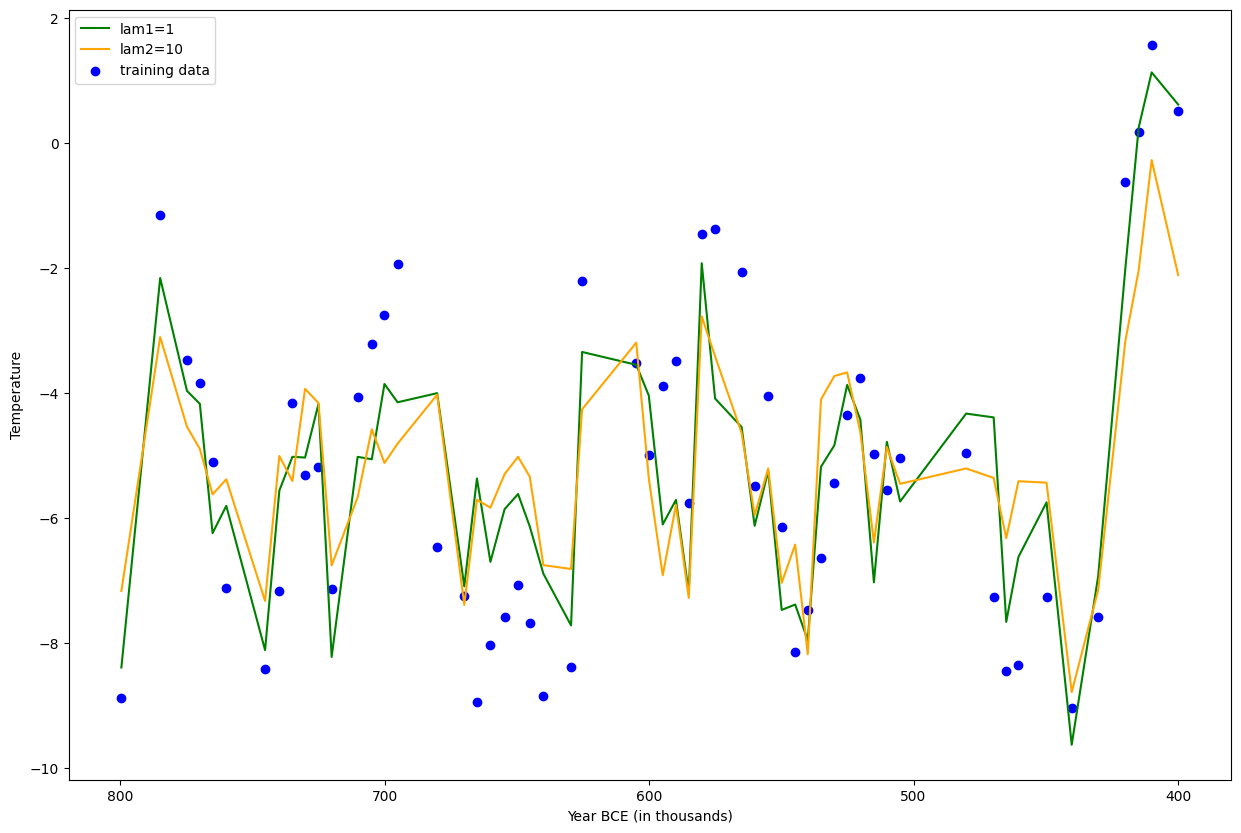
\includegraphics[width=0.9\textwidth]{img_output/p4.5.png}
        \caption*{\textcolor{blue}{Figure 4.5: Regularized basis model}}
        \label{fig:q4.5}
    \end{figure}
    Table 4.5 lists the MSEs corresponding to $\lambda =1,10$ for basis d:
    \begin{table}[H]
        \centering
        \arrayrulecolor{blue}
        \renewcommand{\arraystretch}{1.2} % Adjust row height for readability
    
        \begin{tabular}{|c|c|}
            \hline
            \textbf{\textcolor{blue}{$\bm{\lambda}$}} & \textbf{\textcolor{blue}{MSE}} \\ 
            \hline
            \textcolor{blue}{1} & \textcolor{blue}{30.0606} \\ 
            \textcolor{blue}{10} & \textcolor{blue}{15.6184} \\ 
            \hline
        \end{tabular}
        
        \caption*{\textcolor{blue}{Table 4.5: MSE for different values of $\lambda$ for basis d}}
        \label{tab:mse_comparison}
    \end{table}
    We observe that the regularized regression lines in Figure 4.5 do not fit the training set as well as the unregularized regression line in Figure 3.1(d). Moreover, the $\lambda = 10$ regression line (yellow) in Figure 4.5 does not fit the training set as well as the $\lambda = 1$ regression line (green). However, when we look at the MSEs, we see that the $\lambda = 10$ regression line has the lowest MSE at around 15.62, followed by the $\lambda = 1$ regression line at 30.06, and finally the unregularized ($\lambda = 0$) regression line at 58.95. This tells us that the $\lambda = 10$ line generalizes best, and that the unregularized basis model was overfitting the training set.
    
\end{enumerate}

\end{solution}


%%%%%%%%%%%%%%%%%%%%%%%%%%%%%%%%%%%%%%%%%%%%%
% Name and Calibration
%%%%%%%%%%%%%%%%%%%%%%%%%%%%%%%%%%%%%%%%%%%%%
\clearpage
\subsection*{Name}
\textcolor{blue}{Emma Harris}

\subsection*{Collaborators and Resources}
Whom did you work with, and did you use any resources beyond cs181-textbook and your notes?
\textcolor{blue}{Kevin Liu}


\end{document}
